\section{Cache Invalidation and Replacement Strategies for Location-...}

\subsection{Introduction}

\begin{frame}
\frametitle{Introduction}

	\begin{center}
	\Large
	Published in IEEE Transactions on Computers\\\vspace{1em}
	by\\\vspace{1em}
	Baihua Zheng, Jianliang Xu, and Kik L. Lee\\\vspace{1em}
	October 2002
	\end{center}

\end{frame}


\begin{frame}
\frametitle{Motivation}
\large
Doing location based queries from a mobile phone, with a cache, the user could:
\begin{itemize}
\item Save Money
\item Reduce Network Traffic
\item Conserve battery
\end{itemize}

\vspace{2em}
Existing cache replacement policies too simple. Does not consider valid scopes of cached items
\vspace{0.5em}

\end{frame}


\begin{frame}
\frametitle{Related Work}

Temporal-dependent invalidation
\begin{itemize}
\item server sends \textit{invalidation reports} to clients
\end{itemize}
\vspace{1em}
Location-dependent invalidation
\begin{itemize}
\item Depending on users location or area after movement, data might be invalidated.
\end{itemize}
\vspace{1em}
Semantic data caching
\begin{itemize}
\item cached items saved with locations associated with query
\end{itemize}

\end{frame}

%----------------------------------------------


\subsection{Problem}

\begin{frame}
\frametitle{Problem}

Mobile, cache enabled, clients communicate with fixed hosts, requesting location based service from fixed hosts. 

A Geometric model is used, with identifying their location via e.g. GPS.

\begin{itemize}
\item Mobile clients
\item Fixed hosts
\item Geometric model
\end{itemize}

\vspace{1em}

- Perceived Problem
\begin{quotation}
	Given a cache enabled client and a LBS server, which cache replacement technique performs best, and does data distribution have an effect.
\end{quotation}
\end{frame}


%----------------------------------------------

\subsection{Contribution}
\begin{frame}
\frametitle{Invalidation Strategies}

Location-Dependent Invalidation Strategies
\hspace{1em}

\begin{itemize}
\item[PE\hspace{0.5em}] Polygonal Endpoints
\item[AC\hspace{0.5em}] Approximate Circle
\item[CEB] Cache Efficientcy Based
\end{itemize}

\hspace{1em}

Methods to support invalidation of cache items based on the valid scope of each items 


\end{frame}


\begin{frame}
\frametitle{CEB - Cache Efficientcy Based}


$E(v^{'}_i)=\frac{A(v^{'}_i)/A(v)}{(D+O(v^{'}_i))/D} = \frac{A(v^{'}_i)D}{A(v)(D+O(v^{'}_i))}$

\begin{itemize}
\item $v^{'}_i$ - subregion of $v$
\item $A(v^{'}_i)$ - area of $v^{'}_i$
\item $O(v^{'}_i)$ - overhead to record scope of $v^{'}_i$
\item $D$ - Data size
\item $A(v^{'}_i)/A(v)$ - Cache hit ratio (assuming uniform probability of queries from all locations)
\item $(D+O(v^{'}_i))/D$ - Cost ratio to archive hit ratio
\item $E(v^{'}_i)$ - Caching efficiency of data item with respect to scope of $v^{'}_i$
\end{itemize}

\end{frame}


\begin{frame}
\frametitle{Cache Replacement Policies}

Eject cache items furthest away from user\\
\vspace{1em}
Favor cache items with larger valid scope\\
\vspace{1em}

\begin{itemize}
\item[PA\hspace{1em}] Probability Area $c_{i,j} = P_i * A(v^{'}_{i,j})$
\item[PAID] Probability Area Inverse Distance  $c_{i,j} = \frac{P_i * A(v^{'}_{i,j})}{D(v^{'}_{i,j})}$
\end{itemize}

\begin{itemize}
\item $c_{i,j}$ - Cost function of data value $j$ of cache item $i$
\item $P_i$ - Access probability of cache item
\item $A(v^{'}_{i,j})$ - Area of attached valid scope $v^{'}_{i,j}$
\item $D(v^{'}_i)$ - Distance between user and valid scope $A(v^{'}_{i,j})$
\end{itemize}

\end{frame}


%----------------------------------------------

\subsection{Experimental Results}

\begin{frame}
\frametitle{Setting}


\begin{columns}
	\begin{column}{0.5\textwidth}
		\only<1>{ 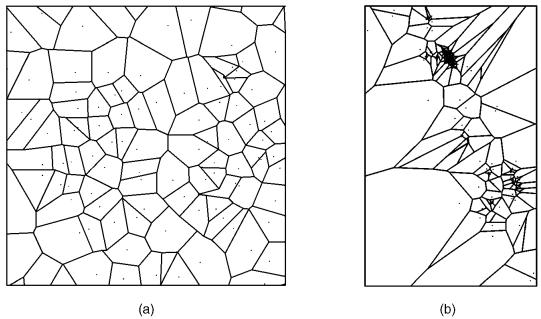
\includegraphics[page=1,scale=0.45]{images/voronoi.jpg}}
	\end{column}
	\begin{column}{0.5\textwidth}
		\begin{itemize}\itemsep 16pt
		\item 2 datasets, modeled as Voronoi Diagrams (110/185 Points)
		\end{itemize}
	\end{column}
\end{columns}
\end{frame}

\begin{frame}

\begin{center}
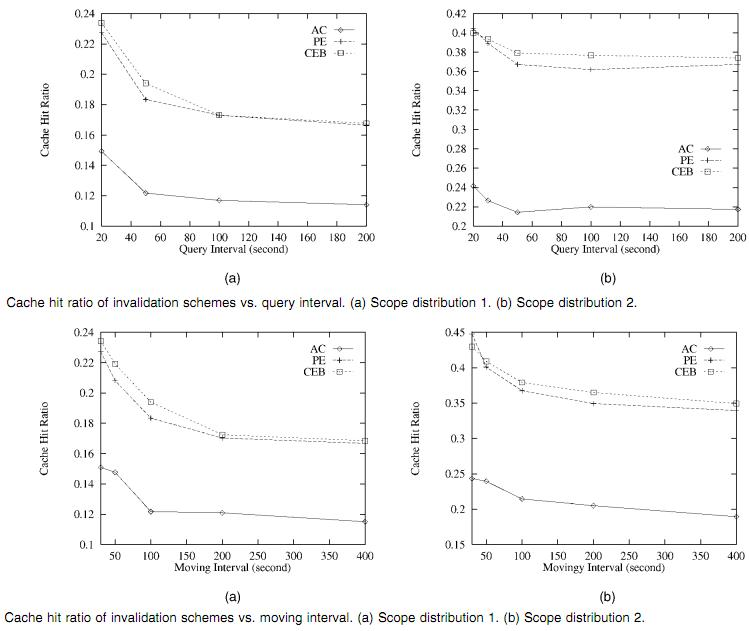
\includegraphics[scale=0.45]{images/fig3-4.jpg}
\end{center}

\end{frame}

\begin{frame}
\frametitle{Cache hit ratio / Data Size - scope 1 and 2}

\begin{center}
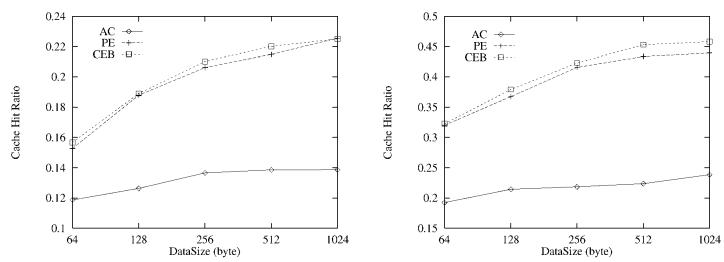
\includegraphics[scale=0.6]{images/fig5.jpg}
\end{center}

\end{frame}

\begin{frame}
\frametitle{Cache hit ratio / Query interval - scope 1 and 2}

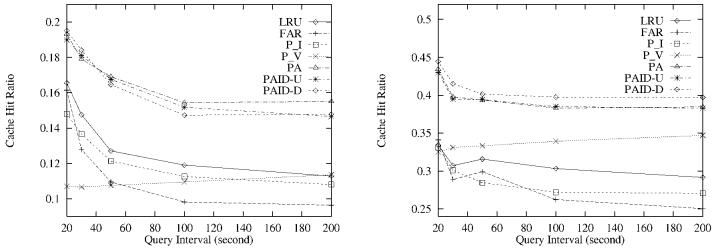
\includegraphics[scale=0.5]{images/fig6.jpg}\\
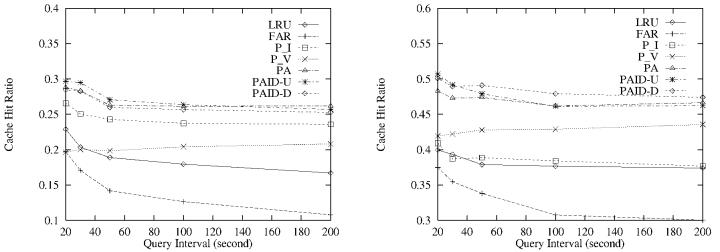
\includegraphics[scale=0.5]{images/fig7.jpg}


\end{frame}

\begin{frame}
\frametitle{Cache hit ratio / Moving interval - scope 1 and 2}

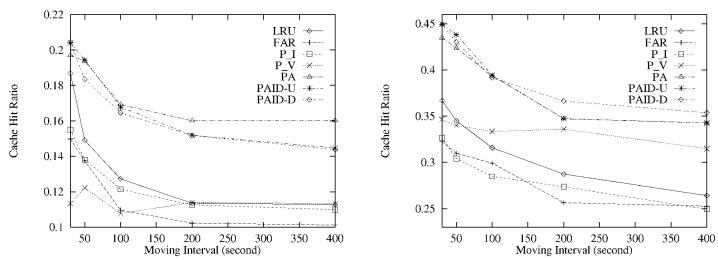
\includegraphics[scale=0.5]{images/fig8.jpg}\\
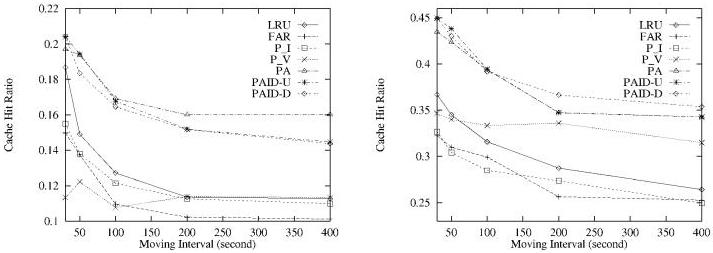
\includegraphics[scale=0.5]{images/fig9.jpg}

\end{frame}


\begin{frame}
\frametitle{Conclusion}
\Large

\textbf{Introduce}
\begin{itemize}
\item CEB
\item PA
\item PAID
\item Data Distance (PAID)
\end{itemize}

Show experimentally that using PA and PAID will give some improvement


\end{frame}

\begin{frame}
\frametitle{Impression}

Paper too long, with very little content\\
\vspace{1em}
Experimental section almost 2/3 of paper.\\
\vspace{1em}
Paper does not state problem to be solved, is a rather just a description of methods\\
\vspace{1em}
Contribution: experimentally showing that obvious improvements to existing ideas works okay.


\end{frame}